%% Supplementary material (J-BHI). Standalone; pdflatex.
\documentclass[journal,onecolumn]{IEEEtran}
\usepackage[T1]{fontenc}\usepackage[utf8]{inputenc}\usepackage{lmodern}\usepackage{amsmath}\usepackage{booktabs}\usepackage{graphicx}
\usepackage{longtable}\usepackage{array}\usepackage{xcolor}\usepackage{adjustbox}\usepackage[hidelinks]{hyperref}
\graphicspath{{../empirical/figures/}{../integrated/figures/}}
\makeatletter\def\input@path{{../empirical/}{../integrated/}{./}}\makeatother
\let\origtable\table\let\endorigtable\endtable
\renewenvironment{table}[1][]{\begin{origtable}[!htbp]}{\end{origtable}} % [1][] absorbs the generated placement option
\renewcommand{\thetable}{S\arabic{table}}\renewcommand{\thefigure}{S\arabic{figure}}
\begin{document}
\title{Supplementary Material for ``Leakage-Safe Evaluation of Machine-Learning Models for Mental-Health Prediction from Actigraphy: Protocol, Benchmark and Appraisal of Published Claims''}
\author{Aminat~Abiola~Ajibola}
\maketitle
\section{Table S1: TRIPOD+AI checklist}
\begingroup\footnotesize\input{supplement_tripod_checklist}\endgroup
\section{Table S2: feature definitions}
\begingroup\footnotesize\input{supplement_features}\endgroup
\section{Tables S3 and S4: identification sources and study list}
\begingroup\footnotesize\input{supplement_part1_sources}\endgroup
% Auto-generated by scripts/part1_figure.py from part1_studies.csv
\begin{table}[!htbp]\centering\caption{Part I seed extraction: published supervised models on the four cohorts identified before the formal search (Supplementary Table S4 lists sources). Red cells are extractions from abstracts that must be verified against the full text during dual extraction; the formal search will add studies to this list.}\label{tab:part1}\scriptsize
\begin{adjustbox}{max width=\linewidth}\begin{tabular}{llllllllll}\toprule
ID & First author & Year & Cohorts & Best model & Split unit & Best reported & Calib. & Ext. val. & Code\\\midrule
S01 & Garcia-Ceja & 2018 & DEPRESJON & Random forest / DNN & participant (leave-one-patient-out) & F1 0.73 & no & no & yes\\
S02 & Zanella-Calzada & 2019 & DEPRESJON & Random forest & day/window & accuracy 0.89 & no & no & no\\
S03 & Frogner & 2019 & DEPRESJON & 1D-CNN & participant (leave-one-participant-out) & \textcolor{red}{F1 verify} & no & no & no\\
S04 & Jakobsen & 2020 & DEPRESJON & Random forest / DNN / CNN & participant (leave-one-out) & \textcolor{red}{accuracy verify} & no & no & no\\
S05 & Jakobsen & 2020 & PSYKOSE & Classical ML & participant (leave-one-patient-out) & \textcolor{red}{F1 verify} & no & no & yes\\
S06 & Hicks & 2021 & HYPERAKTIV & Classical ML & unstated (10-fold on features) & \textcolor{red}{accuracy verify} & no & no & yes\\
S07 & Rodriguez-Ruiz & 2022 & DEPRESJON & 2D-CNN & day/window & accuracy 0.767 & no & no & no\\
S08 & Rodriguez-Ruiz & 2022 & DEPRESJON+PSYKOSE & CNN & day/window & \textcolor{red}{accuracy verify} & no & no & no\\
S09 & Kumar & 2022 & DEPRESJON & ML on autoregressive features & unstated & accuracy 0.78 & no & no & no\\
S10 & Ahmed (arXiv) & 2023 & DEPRESJON & Transfer learning ensemble & \textcolor{red}{modified leave-one-out (verify)} & accuracy 0.96 & no & claims independent set & no\\
S11 & Hybrid RF-ANN (arXiv) & 2023 & DEPRESJON & RF-ANN ensemble & unstated & \textcolor{red}{accuracy verify} & no & no & no\\
S12 & UMAP study & 2023 & DEPRESJON & ML + UMAP & unstated & \textcolor{red}{accuracy verify} & no & no & no\\
S13 & Genetic-algorithm feature selection & 2023 & DEPRESJON & GA feature selection + classifier & day/window (intervals) & \textcolor{red}{accuracy verify} & no & no & no\\
S14 & Attention CNN (IoMT) & 2023 & PSYKOSE & Deep CNN + attention & day/window & \textcolor{red}{accuracy verify} & no & no & no\\
S15 & Multi-branch DL & 2024 & PSYKOSE & Multi-branch deep network & day/window & accuracy 0.92 & no & no & no\\
S16 & DL + XAI & 2024 & PSYKOSE (+DEPRESJON) & Deep network + XAI & day/window (24-h segments) & accuracy 0.94 & no & no & no\\
S17 & Hopping-mean augmentation & 2024 & DEPRESJON & Augmented ML & day/window & \textcolor{red}{accuracy verify} & no & no & no\\
S18 & IoMT dimensionality reduction & 2024 & HYPERAKTIV & 10 classifiers on reduced features & unstated & \textcolor{red}{accuracy verify} & no & no & no\\
S19 & Explainable XGBoost & 2025 & DEPRESJON & XGBoost + ADASYN & \textcolor{red}{unstated in abstract (verify)} & accuracy 0.849 & no & no & no\\
S20 & Improved CNN framework & 2025 & DEPRESJON+PSYKOSE & Improved CNN & \textcolor{red}{day/window (verify)} & \textcolor{red}{accuracy verify} & no & no & no\\
S21 & Enhanced ADHD ML & 2025 & HYPERAKTIV/OBF (45 participants) & SVM & \textcolor{red}{unstated (verify)} & F1 0.779 & no & no & no\\
S22 & HYPERAKTIV ML study & 2025 & HYPERAKTIV & RF / LightGBM / SVM & unstated & \textcolor{red}{accuracy verify} & no & no & no\\
S23 & Multimodal digital biomarkers & 2025 & HYPERAKTIV & Bernoulli NB (actigraphy+HRV) & \textcolor{red}{unstated (verify)} & F1 0.79 & no & no & no\\
S24 & OBF-Psychiatric descriptor & 2025 & OBF-Psychiatric & Classical ML baselines & \textcolor{red}{participant (verify)} & \textcolor{red}{accuracy verify} & no & no & yes\\
S25 & Data-uncertainty case study & 2025 & OBF-Psychiatric (ADHD) & QC + ML & \textcolor{red}{participant (verify)} & nan no difference after QC & no & no & no\\
S26 & ViT / CoAtNet on images & 2025 & DEPRESJON+PSYKOSE & CoAtNet-Tiny & participant (three-fold subject-wise) & \textcolor{red}{accuracy verify} & no & no & no\\
S27 & Time-segmentation evaluation & 2026 & DEPRESJON & ML on day segments & \textcolor{red}{verify} & \textcolor{red}{accuracy verify} & no & no & no\\
S28 & Accurate ADHD identification & 2022 & HYPERAKTIV & ML on real-time activity & \textcolor{red}{unstated (verify)} & \textcolor{red}{accuracy verify} & no & no & no\\
\bottomrule\end{tabular}\end{adjustbox}\end{table}

\section{Table S5: run manifests and prediction files}
Every experiment run writes \path{results/real/<experiment>/manifest.json} (timestamp, git commit and dirty flag, configuration hash and configuration, interpreter and platform, package versions, SHA-256 of every raw file, synthetic flag, experiment name, rows written) and per-window out-of-fold predictions \path{results/real/<experiment>/predictions/<cohort>.<model>.<splitter>.csv} (seed, fold, window\_id, subject\_id, cohort, y, p). Tables are regenerated by \path{python -m mlmh retable}, \path{scripts/part1_figure.py}, \path{scripts/part2_extra_figures.py} and \path{scripts/fill_e*_paragraph.py}.
\section{Table S6: 1D-CNN arm}
% Auto-generated by mlmh.reporting.tables -- do not edit by hand.
\begin{table}[!htbp]
\centering
\caption{E1: discrimination under subject-wise versus record-wise cross-validation. Cells give the estimate on seed-averaged out-of-fold predictions with subject-level BCa 95\% bootstrap intervals; inflation is the paired record-wise minus subject-wise difference.}
\label{tab:e1_e1_cnn}
\footnotesize
\begin{adjustbox}{max width=\linewidth}
\begin{tabular}{llllllll}
\toprule
Cohort & Model & Window AUROC subject-wise & Window AUROC record-wise & Window inflation & Subject AUROC subject-wise & Subject AUROC record-wise & Subject inflation \\
\midrule
depresjon & 1D-CNN & 0.696 [0.576, 0.795] & 0.729 [0.671, 0.784] & 0.033 [-0.063, 0.122] & 0.738 [0.634, 0.844] & 0.912 [0.837, 0.959] & 0.174 [0.067, 0.270] \\
psykose & 1D-CNN & 0.849 [0.744, 0.910] & 0.892 [0.836, 0.935] & 0.043 [-0.000, 0.095] & 0.922 [0.852, 0.976] & 0.986 [0.963, 1.000] & 0.064 [0.016, 0.111] \\
hyperaktiv & 1D-CNN & 0.459 [0.356, 0.588] & 0.513 [0.447, 0.578] & 0.054 [-0.079, 0.189] & 0.455 [0.371, 0.563] & 0.529 [0.432, 0.622] & 0.074 [-0.060, 0.208] \\
\bottomrule
\end{tabular}
\end{adjustbox}
\end{table}
\input{tables/e1_auroc_inflation_subject_e1_cnn}
\section{Table S7: calibration of every model (E3)}
% Auto-generated by mlmh.reporting.tables -- do not edit by hand.
\begin{table}[!htbp]
\centering
\caption{E3: calibration alongside discrimination for every model in E1 (subject-wise arm) and E2, plus logistic recalibration of external predictions.}
\label{tab:e3}
\footnotesize
\begin{tabular}{llrrrrr}
\toprule
Exp. & Run & AUROC & Brier & Cal. slope & Cal. intercept & ECE \\
\midrule
E1 & depresjon.logreg.subject\_wise & 0.779 & 0.187 & 0.69 & -0.51 & 0.102 \\
E1 & depresjon.rf.subject\_wise & 0.770 & 0.181 & 0.77 & 0.01 & 0.056 \\
E1 & depresjon.xgboost.subject\_wise & 0.764 & 0.192 & 0.53 & 0.27 & 0.105 \\
\bottomrule
\end{tabular}
\end{table}

\section{Table S8: ablation (E6)}
% placeholder until E6 completes

\section{Table S9: sex-stratified performance (E4)}
\input{tables/e4_fairness_sex}
\section{Table S10: full window-level metrics (E1)}
% Auto-generated by mlmh.reporting.tables -- do not edit by hand.
\begin{table}[!htbp]
\centering
\caption{E1: window-level discrimination and calibration for every model, cohort and splitting design (mean over seeds).}
\label{tab:e1full}
\footnotesize
\begin{tabular}{llllllllll}
\toprule
Cohort & Model & Split & Accuracy & Macro-F1 & AUROC & Brier & Cal. slope & Cal. intercept & ECE \\
\midrule
depresjon & Majority class & subject-wise & 0.653 & 0.395 & 0.482 & 0.227 & -4.01 & -0.00 & 0.000 \\
depresjon & Majority class & record-wise & 0.653 & 0.395 & 0.499 & 0.227 & 0.29 & 0.00 & 0.000 \\
depresjon & Logistic regression & subject-wise & 0.722 & 0.706 & 0.765 & 0.194 & 0.52 & -0.54 & 0.118 \\
depresjon & Logistic regression & record-wise & 0.761 & 0.750 & 0.840 & 0.163 & 0.90 & -0.62 & 0.095 \\
depresjon & Random forest & subject-wise & 0.724 & 0.679 & 0.762 & 0.185 & 0.69 & 0.01 & 0.061 \\
depresjon & Random forest & record-wise & 0.806 & 0.782 & 0.874 & 0.136 & 1.23 & -0.11 & 0.039 \\
depresjon & XGBoost & subject-wise & 0.722 & 0.676 & 0.745 & 0.202 & 0.43 & 0.29 & 0.123 \\
depresjon & XGBoost & record-wise & 0.802 & 0.776 & 0.872 & 0.137 & 0.82 & 0.07 & 0.039 \\
\bottomrule
\end{tabular}
\end{table}

\section{Figures S1 to S3: ROC and reliability curves}
\begin{figure}[!htbp]\centering
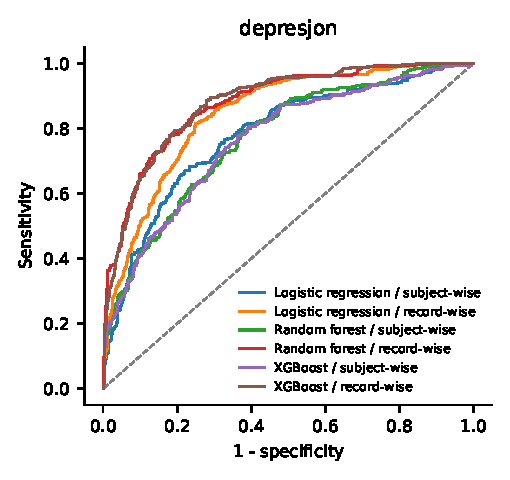
\includegraphics[width=.32\textwidth]{e1_roc_depresjon.pdf}\hfill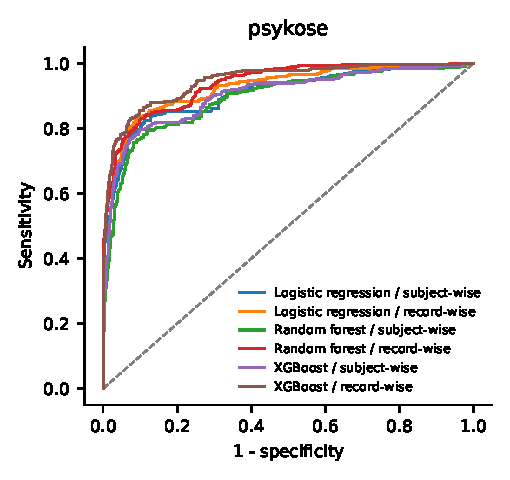
\includegraphics[width=.32\textwidth]{e1_roc_psykose.pdf}\hfill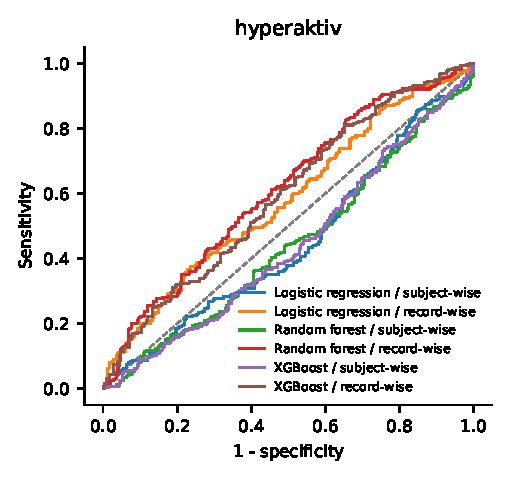
\includegraphics[width=.32\textwidth]{e1_roc_hyperaktiv.pdf}\\[0.4em]
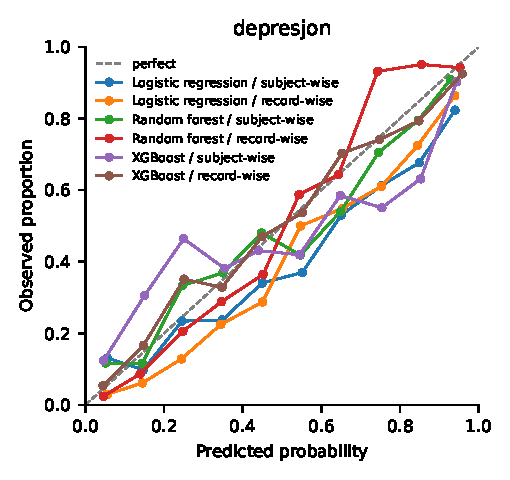
\includegraphics[width=.32\textwidth]{e1_reliability_depresjon.pdf}\hfill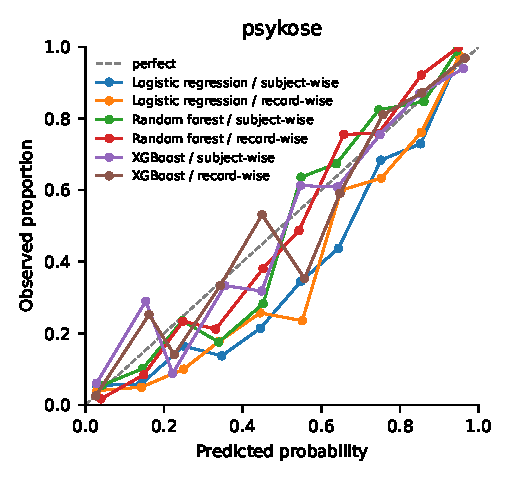
\includegraphics[width=.32\textwidth]{e1_reliability_psykose.pdf}\hfill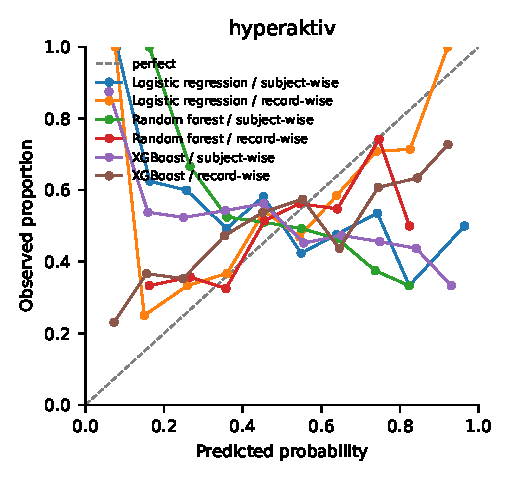
\includegraphics[width=.32\textwidth]{e1_reliability_hyperaktiv.pdf}
\caption{E1. ROC (top) and reliability (bottom) curves per cohort under subject-wise and record-wise cross-validation.}\end{figure}
\begin{figure}[!htbp]\centering
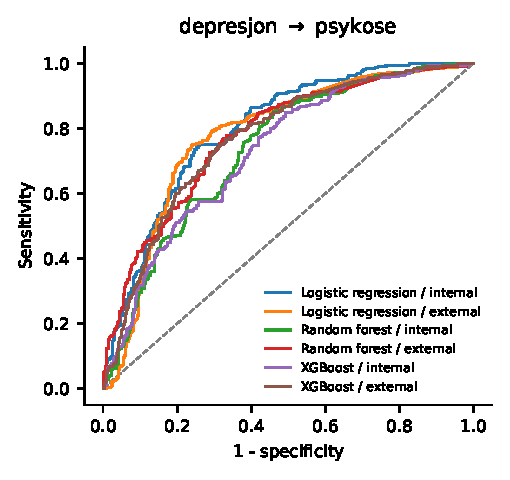
\includegraphics[width=.32\textwidth]{e2_roc_depresjon_to_psykose.pdf}\hfill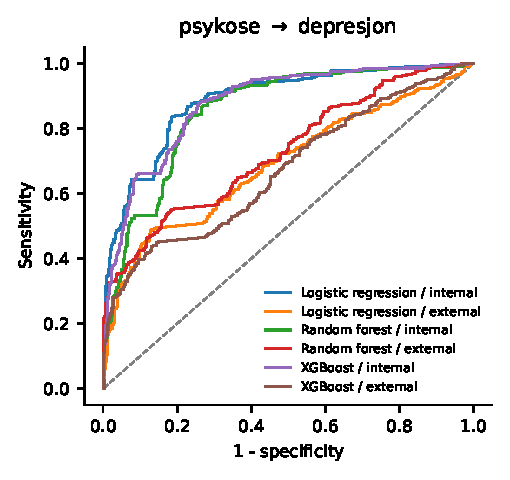
\includegraphics[width=.32\textwidth]{e2_roc_psykose_to_depresjon.pdf}\hfill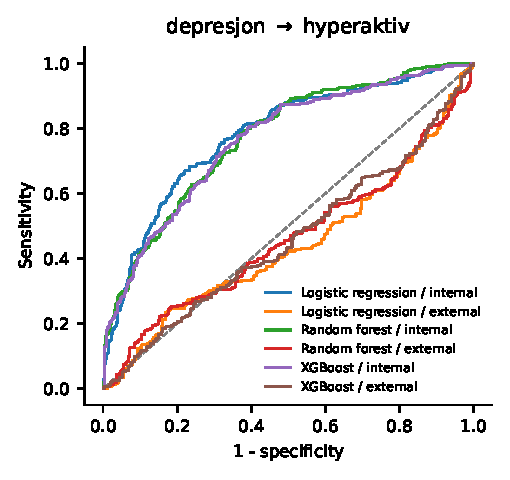
\includegraphics[width=.32\textwidth]{e2_roc_depresjon_to_hyperaktiv.pdf}\\[0.4em]
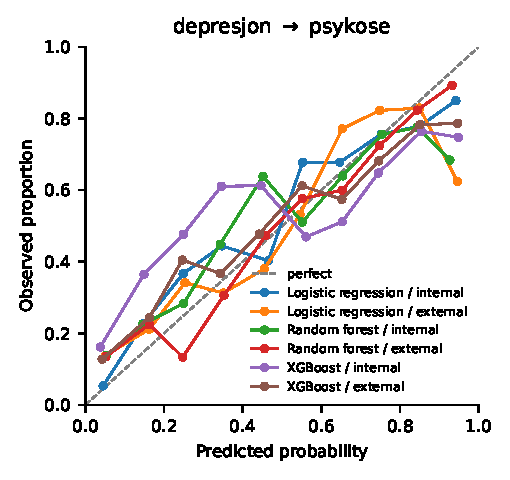
\includegraphics[width=.32\textwidth]{e2_reliability_depresjon_to_psykose.pdf}\hfill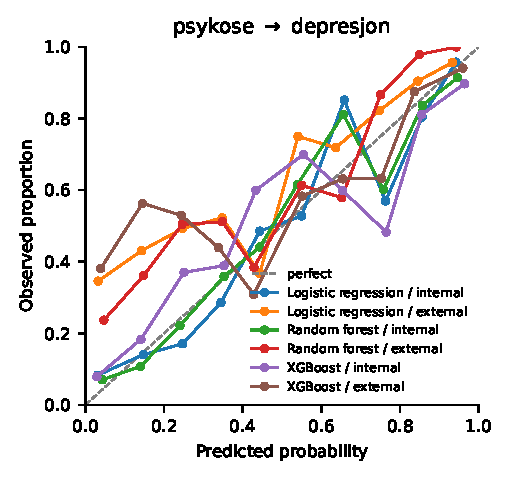
\includegraphics[width=.32\textwidth]{e2_reliability_psykose_to_depresjon.pdf}\hfill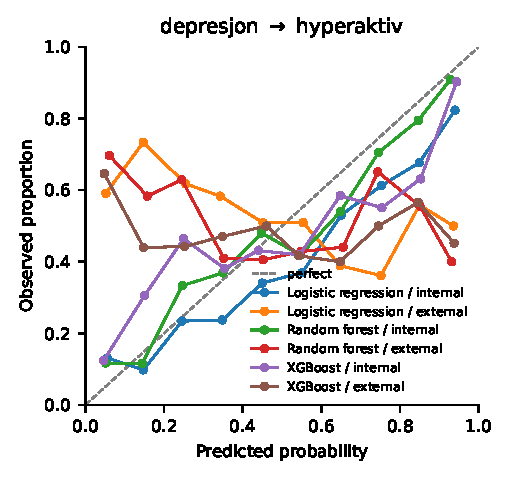
\includegraphics[width=.32\textwidth]{e2_reliability_depresjon_to_hyperaktiv.pdf}
\caption{E2. ROC (top) and reliability (bottom) curves of internal and external predictions per cohort pair.}\end{figure}
\begin{figure}[!htbp]\centering
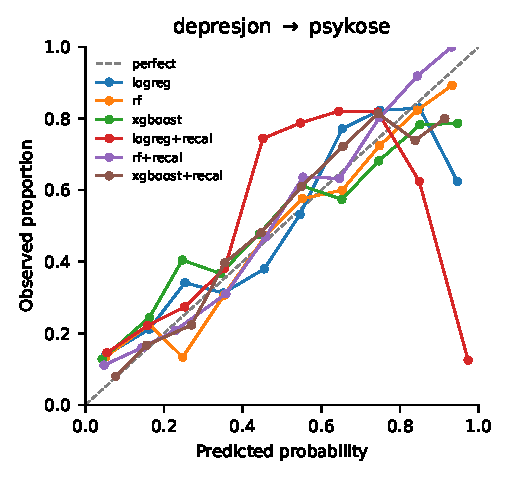
\includegraphics[width=.32\textwidth]{e3_reliability_depresjon_to_psykose.pdf}\hfill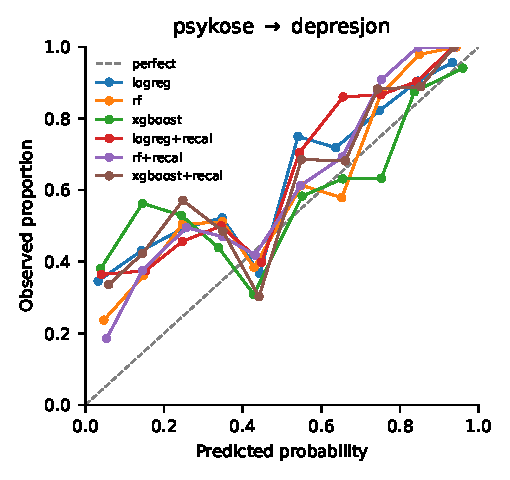
\includegraphics[width=.32\textwidth]{e3_reliability_psykose_to_depresjon.pdf}\hfill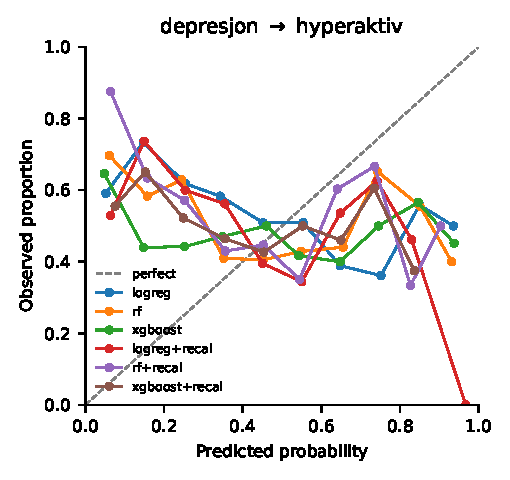
\includegraphics[width=.32\textwidth]{e3_reliability_depresjon_to_hyperaktiv.pdf}
\caption{E3. Reliability of external predictions before and after logistic recalibration fitted on the training cohort.}\end{figure}
\begin{figure}[!htbp]\centering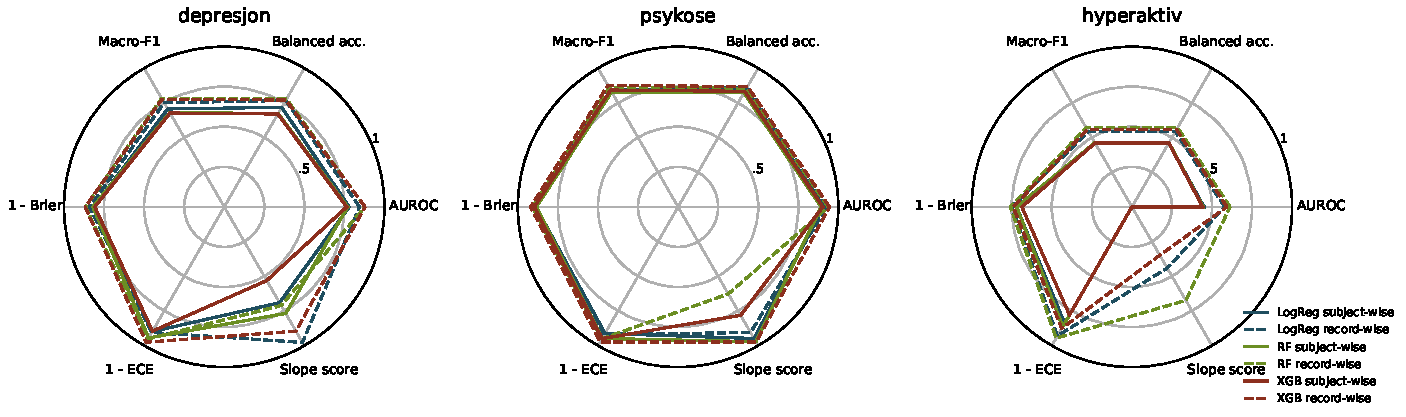
\includegraphics[width=\textwidth]{e1_radar_models.pdf}
\caption{Multi-metric profile of the models per cohort under subject-wise (solid) and record-wise (dashed) cross-validation.}\end{figure}
\end{document}
